In this section are analyzed some known heuristics algorithms for the TSP problem. An heuristic algorithm doesn’t return the optimal solution of the problem but computes a near optimal solution valuing optimality, accuracy, time speed and completeness. Those kinds of algorithms are mainly used when the computational time of the exact algorithms is too high (mainly because of the size of the input instance) and there is no need for an exact solution.

Heuristic Algorithms are divided into three main categories:
\begin{description}
    \item[Constructive Heuristics:] algorithms that iterates to extend a current partial solution until a complete solution is found, trying to make an improvement at each iteration.
    \item[Refinement Heuristics:] starting from a complete solution (not optimal), it rearranges some edges trying to further improve the current solution.
    \item[Metaheuristics:] high level heuristic algorithms mainly used to escape local optimality and to explore a more vast range of possible solutions.
\end{description}

\section{Constructive Heuristics}
\subsection{Greedy: Nearest Neighbor}
Nearest Neighbour it’s a popular greedy algorithm, easy to implement, and that solves the TSP problem in a sub-optimal way. The algorithm \ref{algo:greedy} usually starts with a single starting node and at each iteration it connects the current node to the closest node not already in the path, repeating this operation until all nodes are connected. It’s easy to notice how in general this kind of algorithm won’t find the shortest route and thus his sub-optimality.

\begin{algorithm}
    \caption{Nearest Neighbour}\label{algo:greedy}
    \begin{algorithmic}[1]
    \Require $G = (V,E), c:E \to \mathbb{R}^+, startNode \in V$
    \Ensure $\text{sub optimal TSP solution}$
    \State $visited \gets \left \{ startNode \right \}$
    \State $current \gets startNode$




    \State $solution \gets$ empty
    \State $cost \gets 0$




    \While{$\left | visited \right | \neq \left | V  \right |$}
    \State $candidate \gets *$ find closest node to current $*$
    \State $cost \gets cost + \operatorname{dist}(current, candidate)$
    \State add $candidate$ to $visited$
    \State add ($current$,$candidate$) edge to $solution$
    \State $current \gets candidate$
    \EndWhile




    \State add ($current$,$startNode$) edge to $solution$
    \State $cost \gets cost + \operatorname{dist}(current, startNode)$


    \end{algorithmic}
\end{algorithm}

This algorithm has complexity $O(n^2)$ since it needs to scan at most $n$ nodes for each node in the graph. At fig. \ref{fig:greedy} one can better understand how the algorithm works.

\begin{figure}[!h]
    \centering
    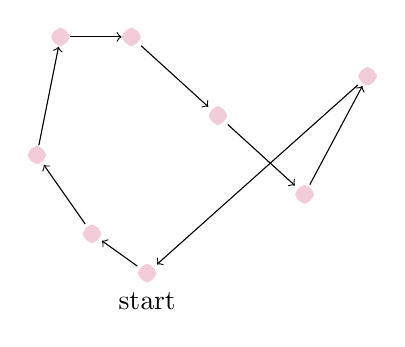
\begin{tikzpicture}
        \tikzstyle{city} = [fill=purple!20,rounded corners]


        \node[city] (A) at (1.3,4.0){};
        \node[city] (B) at (1.6,5.5){};
        \node[city,label=below:start] (C) at (2.7,2.5){};
        \node[city] (D) at (4.7,3.5){};
        \node[city] (E) at (2.0,3.0){};
        \node[city] (F) at (2.5,5.5){};
        \node[city] (G) at (3.6,4.5){};
        \node[city] (H) at (5.5,5){};


        %\draw[->] (C.west) -- (E.east);
        %\draw[->] (B.south) -- (A.east);
        \draw[->] (C) edge (E) (E) edge (A) (A) edge (B) (B) edge (F) (F) edge (G) (G) edge (D) (D) edge (H) (H) edge (C);

    \end{tikzpicture}
    \caption{Example of Nearest Neighbor} \label{fig:greedy}
\end{figure}

To slightly improve this greedy algorithm performance, in our implementation we actually preferred a multistart approach. The algorithm is called multiple times within a time limit and at each iteration a random $startNode$ is used as the starting node. In this way, at each iteration we obtain different solutions with different costs and when the time is up, at the end of the run, only the best solution (the one with minimal cost) is returned in output.

\subsubsection*{The Grasp Variant}
The Greedy Randomized Adaptive Search Procedure (GRASP) is a technique that introduces randomization in the choices of the greedy algorithms.
Applied to the Nearest Neighbor algorithm, it actually works by adding a certain probability value during the running of it and this slightly modifies its behavior of improvement of the current solution.

At each iteration, instead of choosing the nearest node to the current one, we have a certain probability of choosing the second nearest node. That way we can add some randomness to the algorithm and this can actually improve the overall optimality of the final solution.
Obviously even this variant has been implemented and runs similarly to the multistart Nearest Neighbor algorithm within a time limit, and with different starting nodes at each iteration.

\subsection{Extra-Mileage: Farthest Insertion}
The Farthest Insertion heuristic described in algorithm \ref{algo:extramileage}, also called Extra-Mileage heuristic, unlike the Nearest Neighbor algorithm, doesn’t need a starting node, instead starts by connecting the farthest nodes in the graph as an initial cycle. Because of that it is defined as a deterministic method, meaning that it will always return the same solution over the same input instance.

\begin{figure}[!h]
    \centering
    \begin{tikzpicture}
        \tikzstyle{city} = [fill=purple!20,rounded corners]


        \node[city] (A) at (1,5){};
        \node[city] (B) at (2,4){};
        \node[city,label=above:h] (C) at (3,7){};
        \node[city,label=below:j] (D) at (4,1){};
        \node[city,label=above:i] (E) at (6,8){};
        \node[city] (F) at (7,3){};
        \node[city] (G) at (9,6){};


    


        \draw[->] (D) edge[bend right] node [right] {} (E);
        \draw[->] (E) edge[bend right] node [right] {} (D);


        \draw[dashed,->] (E) edge (C) (C) edge (D.west);


    


    \end{tikzpicture}
    \caption{Example of Farthest Insertion} \label{fig:extra}
\end{figure}

\begin{algorithm}[h!]
    \caption{Farthest Insertion}\label{algo:extramileage}
    \begin{algorithmic}[1]
    \Require $G = (V,E), c:E \to \mathbb{R}^+$
    \Ensure $\text{sub optimal TSP solution}$


    \State $solution \gets$ empty
    \State $cost \gets 0$
    \State $visited \gets  *$ find diameter nodes i-j of G $*$
    \State add ($i$,$j$) and ($j$,$i$) edges to $solution$
    \State $cost \gets cost + 2 c_{ij}$
   




    \While{$\left | visited \right | \neq \left | V  \right |$}
    \State $candidate \gets $ generic node h $ \notin visited$
    \State $candidate \gets *$ find edge i-j visited that minimizes $\Delta = c_{ih} + c_{hj} - c_{ij}*$
    \State $cost \gets cost + \Delta$
    \State remove ($i$,$j$) edge to $solution$
    \State add ($i$,$h$) and ($h$,$j$) edges to $solution$
    \State add $candidate$ to $visited$


    \EndWhile






    \end{algorithmic}
\end{algorithm}

The first cycle is initialized using the diameter nodes of the graph, then the algorithm continues by looking for a non selected node as in figure \ref{fig:extra} that if inserted in the solution would result in a lower cost tour than the current one.
That simple metric is computed by testing each non visited node with each possible already existing edge, and then keeping the one with lowest $\Delta = c_{ih} + c_{hj} - c_{ij}$.

The Farthest Insertion algorithm has a worst-case time complexity of $O(n^2)$, where $n$ is the number of nodes. However, it has been shown to perform well in practice and can often produce high-quality solutions that are close to optimal for small and medium-sized instances of the TSP.

\section{Refinement Heuristics}
\subsection{2-OPT Refining}
One of the most popular heuristic algorithms for solving the TSP is the 2-opt algorithm.
The 2-opt algorithm is a local search algorithm that iteratively improves an initial tour by swapping pairs of edges to reduce the length of the tour. The algorithm starts by generating an initial tour, such as one produced by the Nearest Neighbor or Farthest Insertion algorithm. It then repeatedly examines all possible pairs of edges in the tour, and if swapping a pair of edges will reduce the length of the tour, the edges are swapped.

More specifically, the 2-opt algorithm works as follows: first, it generates an initial solution, in our implementation we choose to generate it using the multistart Nearest Neighbor algorithm paired with a GRASP approach. It then examines all pairs of edges $(a,a')$ and $(b,b')$, where $a,a',b$ and $b'$ are distinct nodes. If swapping the edges $(a,a')$ and $(b,b')$ will result in a shorter tour, the edges are swapped, and the algorithm continues to search for other pairs of edges to swap. This process is repeated until no further improvements can be made to the tour or until the time limit permits.

To know that a certain swap results in a better solution, the algorithm computes $\Delta \operatorname{c}(a,b) = (c_{ab} + c_{a'b'}) - (c_{aa'} + c_{bb'})$ and if it is negative then we found some good candidates, meaning that the new candidates edges would be shorter than the current ones.

After the swap, the algorithm then changes the order of the successor in the tour to make $b$ connect to $a$ and obtain a new solution, as in fig \ref{fig:2OPT}.

\begin{figure}[!h]
    \centering
    \begin{tikzpicture}
        \tikzstyle{city} = [fill=purple!20,rounded corners]
    
    
        \node[city,label=above:a] (A) at (1,5){};
        \node[city,label=below:b] (B) at (1,1){};
        \node[city,label=above:b'] (C) at (5,5){};
        \node[city,label=below:a'] (D) at (5,1){};
    
    
        \node[city,label=above:a] (E) at (7,5){};
        \node[city,label=below:b] (F) at (7,1){};
        \node[city,label=above:b'] (G) at (11,5){};
        \node[city,label=below:a'] (H) at (11,1){};
    
    
       
    
    
        \draw[dashed,->] (C) edge[bend right] node [right] {} (A);
        \draw[dashed,->] (D) edge[bend left] node [left] {} (B);
    
    
        \draw[dashed,->] (G) edge[bend right] node [right] {} (E);
        \draw[dashed,->,red] (F) edge[bend right] node [left] {} (H);
    
    
        \draw[->] (A) -- (D);
        \draw[->] (B) -- (C);
    
    
        \draw[->] (E) -- (F);
        \draw[->] (H) -- (G);
       
    
    \end{tikzpicture}
    \caption{Example of 2-OPT} \label{fig:2OPT}
\end{figure}

The 2-opt algorithm is known to be effective in practice, and it has been used to solve many large-scale instances of the TSP. The algorithm is relatively efficient, with a time complexity of $O(n^2)$, where $n$ is the number of nodes in the graph.

The same idea goes behind the more general k-OPT Refining algorithm, where instead of swapping only 2 edges at the time, k edges are selected and swapped. For example, 3-opt involves swapping three edges in the tour, while 4-opt involves swapping four edges. By considering larger sets of edges, k-opt can potentially find more optimal solutions than 2-opt, but it is also computationally more expensive.
\begin{algorithm}[h!]
    \caption{2-OPT}\label{algo:2-OPT}
    \begin{algorithmic}[1]
    \Require $G = (V,E), c:E \to \mathbb{R}^+$
    \Ensure $\text{sub optimal TSP solution}$


    \State $solution \gets$ GRASP()
    \State $cost \gets$ cost\textunderscore grasp()
    

    \While{$ !time\textunderscore expired  $}
    \State $\Delta\textunderscore temp \gets$ 0
    \State $edge\textunderscore 1 \gets$ empty
    \State $edge\textunderscore 2 \gets$ empty
    \ForEach {$(a,a') \in E $ }
        \ForEach {$(b,b') \neq (a,a')\in E $}
        \State $\Delta \operatorname{c}(a,b) \gets$  $(c_{ab} + c_{a'b'}) - (c_{aa'} + c_{bb'})$
        \If{$\Delta\textunderscore temp  > \Delta \operatorname{c}(a,b) $}
        \State $edge\textunderscore 1 \gets$ (a,a')
        \State $edge\textunderscore 2 \gets$ (b,b')
        \State $\Delta\textunderscore temp \gets$ $\Delta \operatorname{c}(a,b)$
        \EndIf
        \EndFor
    \EndFor
    
    \If{ $\Delta\textunderscore temp  <0$}
    \State $swap(edge\textunderscore 1,edge\textunderscore 2) $ // swap the selected (a,a'), (b,b') as shown in figure \ref{fig:2OPT}
    \State $cost \gets  $ $cost$ + $\Delta\textunderscore temp$
    \EndIf
    

    \EndWhile

    \end{algorithmic}
\end{algorithm}



\section{Metaheuristics}
\subsection{Variable Neighborhood Search}
The Variable Neighborhood Search (VNS), proposed by Mladenović and Hansen in 1997,  is a metaheuristic optimization algorithm used to solve combinatorial optimization problems. The basic idea of VNS is to iteratively apply a perturbation operator to the current solution and then perform a local search around the perturbed solution. VNS is known for its flexibility and ability to escape from local optima by exploring different neighborhood structures.
In our implementation the VNS algorithm tries to improve the solution made by the 2-opt algorithm. In order to try to escape from the local minima produced by the 2-opt, the algorithm performs for two times a random swap of 5 edges. 
Then it reapplies the 2-opt procedure and if it finds a better solution it updates the global solution.
The overall procedure is applied until a certain time limit is reached.
The algorithm requires O(n) time for each kick, because after the swap operation we have to update the structure that contains all the nodes of the graph. We have also to sum the time required by the 2-opt algorithm. This time at the end has to be multiplied by the number of iterations that this procedure is performed. 

\begin{algorithm}[h!]
    \caption{VNS}\label{algo:VNS}
    \begin{algorithmic}[1]
    \Require $G = (V,E), c:E \to \mathbb{R}^+$
    \Ensure $\text{sub optimal TSP solution}$


    \State $solution \gets$ 2-opt()
   
   
    \While{$ !time\textunderscore expired$}
    \State kick(solution) 
    \State kick(solution)  
    \State $ solution \gets $ 2-opt(solution)
    
    
    \If{cost(solution) < cost(best\textunderscore solution)}
    \State $ best\textunderscore solution \gets$ solution
    \EndIf
    

    \EndWhile

    \end{algorithmic}
\end{algorithm}



\subsection{Tabu}
Tabu search is based on the concept of "tabu" which means "prohibited" or "forbidden". The algorithm maintains a tabu list that keeps track of recent moves that are prohibited from being repeated. 
Tabu search is known for its ability to find good-quality solutions in a relatively short amount of time, although it does not guarantee finding the optimal solution.
The algorithm starts with an initial solution, which can be generated randomly or by using a construction heuristic. In our implementation the initial solution is generated by the grasp heuristic.
In our case at every iteration of the algorithm we select the pair of edges that have the minimum value of delta (delta= as in 2 opt). In this case it doesn't matter if the delta is negative or positive, we only took the minimum delta of the nodes that are not marked as “tabu”.  Then after every swap we select in a random way one of the four nodes involved in the swap operation, and it is inserted into the “tabu” list.
The tabu list is updated during the search process to prevent cycling, which is repeatedly revisiting the same solutions. This allows tabu search to diversify the search and explore different regions of the solution space. Thanks to this feature the algorithm can move around the solution space, avoid being stuck in local minimum, and so try to find a better solution value.
In order to implement the tabu list we create a list of length equals to the number of the nodes of the graph. Every time a node is selected to be a “tabu node” we set it corespective element of the list equals to the number of the current iteration. Then this node cannot be involved in any swap operations until the number of the next iterations have overcome the value of a parameter called “Tmax”. This parameter indicates the number of iterations for which the various nodes selected as forbidden cannot be selected in a swap operation.
The value of Tmax is equivalent to the minimum between 100 and the number of nodes divided by 10.
Each swap requires time equal to O(n) to rearrange the array containing the actual solution. So the overall complexity is equal to O(n*number of swaps).
The algorithm stops its iteration after a given time limit.



\subsection{Simulated Annealing}

Simulated annealing is a metaheuristic optimization algorithm that can be used to solve the Traveling Salesman Problem (TSP).
The name of the algorithm comes from annealing in metallurgy, a technique involving heating and controlled cooling of a material to alter its physical properties. This technique usually archives an approximate solution to the global minimum.
The algorithm starts with an initial solution, which can be generated randomly or using a heuristic, in our case we use the output of the Grasp heuristic as the initial solution.
The algorithm at each iteration selects in a random way two edges (a,a'),(b,b'), where $a,a',b$ and $b'$ are distinct nodes. Then swap it (as shown in figure \ref{fig:2OPT} ) depending on a probability function that depends on a parameter called Temperature (T).
In our implementation the initial value for the temperature is equal to the Cost of the solution found by the grasp algorithm, split by the number of nodes of the instance of the current TSP problem. At each iteration the temperature is multiplied by a factor alpha equals to 0.99. If the algorithm keeps going after 100 iterations, the temperature is set to its initial value.
At each iteration the algorithm checks $\Delta \operatorname{c}(a,b) = (c_{ab} + c_{a'b'}) - (c_{aa'} + c_{bb'})$, that is the new cost of swapping the two edges, clearly this parameter delta may be positive or negative. If the value of delta is negative, that is swapping the two edges the value of the solution is better, the algorithm makes the swap. Otherwise if the value of delta is positive the exchange depends on the value of the following probability function: $e^{\frac{-\Delta \operatorname{c}(a,b)}{T}}$.
Each swap requires time equal to O(n) to rearrange the array containing the actual solution. So the overall complexity is equal to O(n*number of swaps).
The algorithm stops its iteration after a given time limit.

	
\begin{algorithm}[h!]
    \caption{Simulated annealing}\label{algo:SimulatedAnnealing}
    \begin{algorithmic}[1]
    \Require $G = (V,E), c:E \to \mathbb{R}^+$
    \Ensure $\text{sub optimal TSP solution}$


    \State $solution \gets$ GRASP()
    \State $cost \gets$ cost\textunderscore grasp()
    \State $T \textunderscore initial \gets  $ cost/$|$V$|$ 
    \State $T \gets  $ T\textunderscore initial
    \State $ \alpha \gets $ 0.99
    \State $ iteration \gets $ 0
   




    \While{$ !time\textunderscore expired$}
    \State $(a,a') \gets $ random edge
    \State $(b,b') \gets $ random edge 
    \State $p \gets $ random(0,1) // random value from 0 to 0.99
    \State $\Delta \operatorname{c}(a,b) \gets$  $(c_{ab} + c_{a'b'}) - (c_{aa'} + c_{bb'})$
    
    \If{ p $\leq$ $e^{\frac{-\Delta \operatorname{c}(a,b)}{T}}$}
    \State $cost \gets$ cost + $\Delta \operatorname{c}(a,b) $
    \State $swap(a,b)$ // swap the edge as shown in figure \ref{fig:2OPT}
    \EndIf
    \State $T \gets $ T*$\alpha$
    \State $iteration \gets $ iteration + 1
    \If{ iteration $\geq$ 100}
    \State $T \gets  $ T\textunderscore initial
    \State $iteration \gets  $ 0
    \EndIf
    

    \EndWhile

    \end{algorithmic}
\end{algorithm}


